%!TEX program = xelatex
\documentclass[cn,hazy,blue,normal,14pt]{elegantnote}
\usepackage{listings}
\usepackage{minted} 
\usepackage{graphicx}
\usepackage{tikz}
\title{Notes of Andrew-Ng Machine Learning}
\author{MZC}
\begin{document}
\maketitle
\tableofcontents
\newpage
\section{引言}
一个程序被认为能从经验E中学习,解决任务T,达到性能度量值P,当且仅当,有了经验E后,经过P评判,程序在处理T时的性能有所提升。

常用的学习方式有监督学习和无监督学习。
\subsection{监督学习}
\begin{example}
一个学生收集了一些房价的数据。你把这些数据画出来,看起来是这个样子:横轴表示房子的面积,单位是平方英尺,纵轴表示房价,单位是千美元。那基于这组数据,假如你有一个朋友,他有一套750平方英尺房子,现在他希望把房子卖掉,他想知道这房子能卖多少钱。
\end{example}

\begin{example}
给出一个数据集,包含肿瘤大小和其是否是恶性肿瘤,现得知一个肿瘤的大小,判断其是否是恶性肿瘤(或预测概率)。
\end{example}
\begin{definition}[监督学习]
利用一组已知类别的样本调整分类器的参数,使其达到所要求性能的过程称作监督学习。
\end{definition}
\subsection{无监督学习}
相比于监督学习,无监督学习不给出数据的标签,旨在找出数据的某种“结构”,例如聚类算法(cluster algorithm)。
\section{线性回归} 
\subsection{假说表示}
例子同1.1,并把给出的数据集称作训练集,用$m$表示训练样本的数目。
\newpage
\begin{itemize}
    \item $m$代表训练集中实例的数目 
    \item $x$代表输入特征/输入变量
    \item $y$代表目标变量/输出变量
    \item $(x,y)$表示训练集中的实例
    \item $(x^{(i)},y^{(i)}$表示第$i$个观察实例
    \item $h$表示算法的解决方案/函数(hypothesis)
\end{itemize}
单变量线性回归:
$$
h_\theta(x)=\theta_0+\theta_1x
$$
\subsection{代价函数}
如何选择最合适的参数?使建模误差的平方和最小。

\begin{definition}[代价函数]
$$
J(\theta)=\frac{1}{2m}\sum_{i=1}^m(h_\theta(x^{(i)}-y^{(i)})^2
$$
\end{definition}

目标是
$$
\mathop{\text{minimize}}\limits_\theta J(\theta)
$$
\subsection{梯度下降}
梯度下降背后的思想是:开始时我们随机选择一个参数的组合\\$(\theta_0,\cdots,\theta_n)$,计算代价函数,然后我们寻找下一个能让代价函数值下降最多的参数组合。我们持续这么做直到到到一个局部最小值(local minimum),因为我们并没有尝试完所有的参数组合,所以不能确定我们得到的局部最小值是否便是全局最小值(global minimum),选择不同的初始参数组合,可能会找到不同的局部最小值。

批量梯度下降(batch gradient descent):重复下列操作直至收敛。
$$
\theta_j:=\theta_j-\alpha \frac{\partial}{\partial \theta_j}J(\theta)
$$
对于单变元线性回归,$j=0$或$1$。

其中$\alpha$是学习率(learning rate),它决定了我们沿着能让代价函数下降程度最大的方向向下迈出的步子有多大。如果$\alpha$太小,迭代次数过多,程序运行慢;$\alpha$过大时,梯度下降可能越过最低点,导致无法收敛。一般尝试$0.01,0.03,0.1,0.3,1,3,10$。

$j=0$时:
$$
\frac{\partial}{\partial \theta_0}J(\theta)=\frac{1}{m}\sum_{i=1}^m(h_\theta(x^{(i)}-y^{(i)})
$$

$j\neq0$时:
$$
\frac{\partial}{\partial \theta_1}J(\theta)=\frac{1}{m}\sum_{i=1}^m(h_\theta(x^{(i)}-y^{(i)})\times x^{(i)}
$$
\subsection{多变量线性回归}
\begin{definition}[多变量线性回归模型]
$$
h_\theta(x)=\theta_0+\sum_{i=1}^n\theta_ix_i=\theta^TX
$$
其中$X$是一个$m\times(n+1)$的矩阵。
\end{definition}

\noindent 代价函数:
$$
J(\theta_0,\theta_1,\cdots,\theta_n)=\frac{1}{2m}\sum_{i=1}^{m}(h_\theta(x^{(i)})-y^{(i)})^2
$$

\noindent 梯度下降:
$$
\begin{aligned}
 \theta_j :&=\theta_j-\alpha\frac{\partial}{\partial \theta_j}J(\theta_0,\theta_1,\cdots,\theta_n) \\
:&=\theta_j-\frac{\alpha}{m}\sum_{i=1}^{m}(h_\theta(x^{(i)})-y^{(i)}) \cdot x_j^{(i)}   
\end{aligned}
$$
\newpage
\subsubsection{特征缩放和多项式回归}
某些特征可能数量级相差过大导致难以收敛,解决的方法是尝试将所有特征的尺度都尽量缩放到-1到1之间。最简单的方法是令:$x_n=\frac{x_n-\mu_n}{s_n}$,其中$\mu_n$是平均值,$s_n$是标准差。

线性回归并不适用于所有数据,有时我们需要曲线来适应我们的数据,通常我们需要先观察数据然后再决定准备尝试怎样的模型。如需要二次方模型:$h_\theta(x)=\theta_0+\theta_1x_1+\theta_2 x_2^2$,此时可令$x_2=x_2^2$ 来转化成线性回归。

\begin{note}
  如果我们采用多项式回归模型,在运行梯度下降算法前,特征缩放非常有必要。
\end{note}
\subsection{正规方程}
\begin{lemma}
$$
\frac{\partial \theta^TA\theta}{\partial \theta}=(A+A^T)\theta
$$
\end{lemma}
\begin{proof}
令
$$
A=
\begin{bmatrix}
    a_1^1 &\cdots & a_1^n \\
    \vdots &\ddots & \vdots \\
    a_n^1 & \cdots & a_n^n
\end{bmatrix}
$$
则:
$$
\theta^TA\theta=\sum_{j=1}^{n}[\theta_j \sum_{i=1}^{n}(a_i^j\theta_i)]
$$
因此
$$
\frac{\partial \theta^TA\theta}{\partial \theta}=\frac{\partial \sum\limits_{j=1}^{n}[\theta_j \sum\limits_{i=1}^{n}(a_i^j\theta_i)]}{\partial 	\theta}
$$

$$
\frac{\partial \sum\limits_{j=1}^{n}[\theta_j \sum_{i=1}^{n}\limits(a_i^j\theta_i)]}{\partial \theta_q}=2\theta_qa_q^q+\sum_{i=0,i \neq q}^{n}a_i^q\theta_i+\sum_{j=0,j\neq q}^{n}a_q^j\theta_j
$$
$$
\therefore \theta_q'=\begin{bmatrix}
    a_q^1+a_1^q,a_q^2+a_2^q,\cdots,a_n^q+a_q^n
\end{bmatrix}
\begin{bmatrix}
    \theta_1 \\
    \theta_2 \\
    \vdots \\
    \theta_n
\end{bmatrix}
$$
$$
\therefore \frac{\partial \theta^TA\theta}{\partial \theta}=(A+A^T)\theta
$$
\end{proof}
\noindent 令 $A=X^TX$,则有:
$$
\frac{\partial \theta^TX^TX\theta}{\partial \theta}=2X^TX\theta
$$
\begin{lemma}
$$
\frac{\partial X^TA}{\partial X}=A
$$
\end{lemma}
\begin{proof}
$$
X^TA=\begin{bmatrix}
    \sum\limits_{i=1}^{n} x_i a_{1i},\cdots,\sum\limits_{i=1}^{n}x_i a_{ni}
\end{bmatrix}
$$
$$
\frac{\partial X^TA}{\partial X}=\begin{bmatrix}
    a_{11} &\cdots & a_{1n} \\
    \vdots &\ddots & \vdots \\
    a_{n1} &\cdots & a_{nn} 
\end{bmatrix}=A
$$
\end{proof}
\noindent 因此
$$
\frac{\partial \theta^TX^TY}{\partial \theta}=X^TY
$$
\begin{lemma}
$$
\frac{\partial AX}{\partial X}=A^T
$$
\end{lemma}
\noindent 因此
$$
\frac{\partial Y^TX\theta}{\partial \theta}=X^TY
$$
\begin{theorem}
使代价函数最小的$\theta$满足:
$$
\theta=(X^TX)^{-1}X^TY
$$
\end{theorem}
\begin{proof}
$$
\begin{aligned}
  J(\theta)&=\frac{1}{2m}\sum_{i=1}^{m}(x^{(i)}\theta^T-y^{(i)})^2  \\
  &=\frac{1}{2m}(X\theta-Y)^T(X\theta-Y) \\
  &=\frac{1}{2m}(\theta^TX^TX\theta-\theta^TX^TY-Y^TX\theta+Y^TY)
\end{aligned}
$$
\noindent 令:
$$
\Delta=\frac{1}{2m}[\frac{\partial \theta^TX^TX\theta}{\partial \theta}-\frac{\partial \theta^TX^TY}{\partial \theta}-\frac{\partial Y^TX\theta}{\partial \theta}+\frac{\partial Y^TY}{\partial \theta}]
$$
\noindent 根据上述引理:
$$
\Delta=\frac{1}{m}(X^TX\theta-X^TY)
$$
令$\Delta=0$,证毕.
\end{proof}

\begin{table}[h]
\begin{tabular}{|l|l|}
\hline
\textbf{梯度下降}    & \textbf{正规方程}                                                      \\ \hline
需要多次迭代           & 一次运算得出                                                             \\ \hline
需要选择学习率$\alpha$  & 不需要                                                                \\ \hline
当特征数量$n$大时也能较好适用 & 当$n$小于10000 时可以接受                                                  \\ \hline
适用于各种类型的模型       & \begin{tabular}[c]{@{}l@{}}只适用于线性模型,不适合逻辑回归\\ 模型等其他模型\end{tabular} \\ \hline
\end{tabular}
\end{table}
\begin{note}
如果$X^TX$不可逆,那么可以用$\text{pinv}(X^TX)$来代替inv;如果向量的特征太多,导致$m\leqslant n$,可以删除某些特征或者使用正则化。
\end{note}
\section{逻辑回归}
\begin{example}[分类问题]
给出数据集:\{电子邮件,是否为垃圾邮件\},训练一个程序来判断一封邮件是否是垃圾邮件。
\end{example}
我们将因变量(dependent variable)可能属于的两个类分别称为负向类(negative class)和正向类(positive class),则因变量$y\in \{0,1\}$,其中 0 表示负向类,1 表示正向类。期望得到一个函数,输出值在0和1之间,如果$h_\theta(x)\geqslant 0.5$,那么判断其为正向类;$h_\theta(x)<0.5$则判断其为负向类。
\subsection{假说表示}
\begin{definition}[逻辑回归模型]
$$
h_\theta(x)=g(\theta^TX)
$$
其中$X$代表特征向量,$g$代表逻辑函数,一个常用的逻辑函数是Sigmoid function:
$$
g(z)=\frac{1}{1+e^{-z}}
$$
\end{definition}
% \begin{figure}[h]

% \centering

% 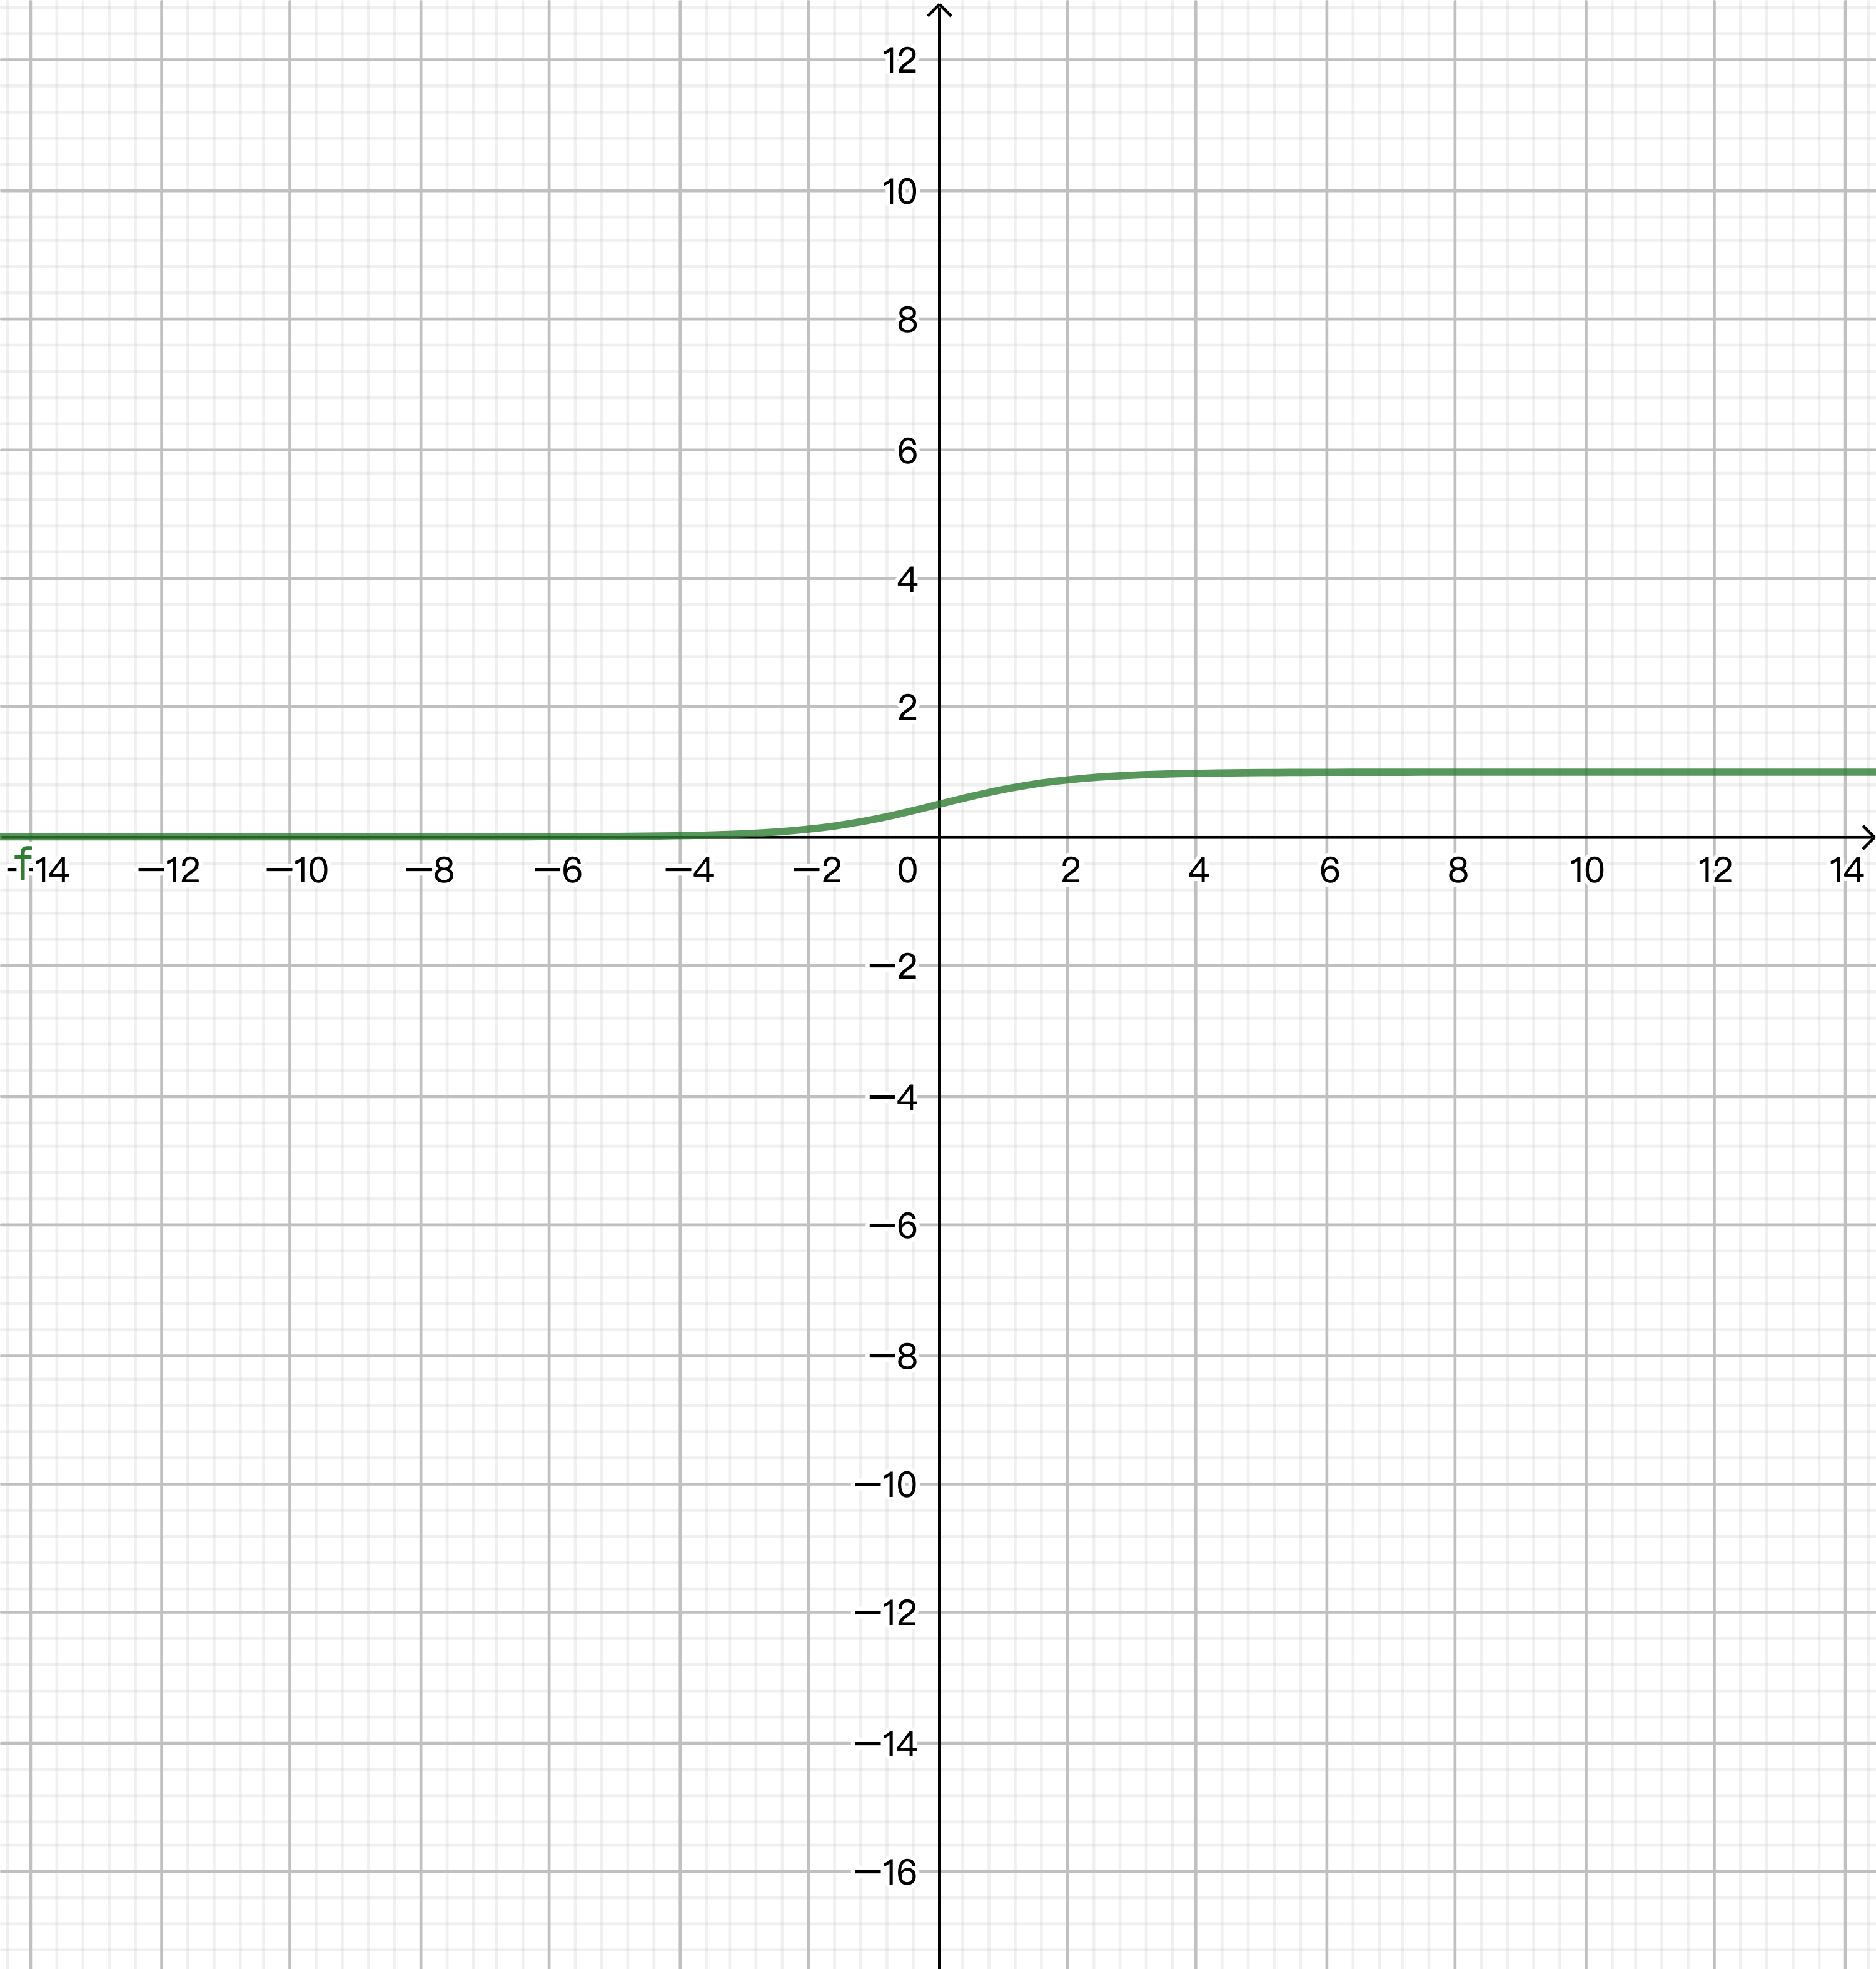
\includegraphics[width=5cm,height=6cm]{image/sigmoid function.png}

% \caption{sigmoid function}

% \end{figure}
\begin{figure}[h]
\begin{center}
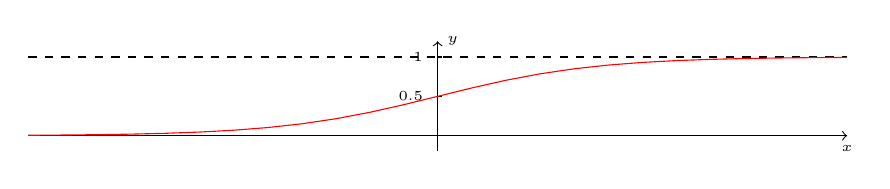
\begin{tikzpicture}
\draw[->](-5.2,0)--(5.2,0)node[left,below,font=\tiny]{$x$};
\draw[->](0,-0.2)--(0,1.2)node[right,font=\tiny]{$y$};
\draw[dashed](-5.2,1)--(5.2,1);
\foreach \y in {0.5,1}{\draw(0,\y)--(0.05,\y)node[left,outer sep=2pt,font=\tiny]at(0,\y){\y};}
\draw[color=red ,domain=-5.2:5.2]plot(\x,{1/(1+(e^(-1*(\x))))});
\end{tikzpicture}
\end{center}
\caption{Sigmoid Function}
\end{figure}
\subsection{代价函数}
如果定义代价函数是模型误差的平方和,那么代价函数将是\textbf{非凸}的(non-convex function),这意味着我们的代价函数有许多局部最小值,这将影响梯度下降算法寻找全局最小值。

因此我们重新定义代价函数:
$$
Cost(h_\theta(x),y)=\begin{cases}
    -\log(h_\theta(x)) & \text{if}\quad  y=1 \\
    -\log(1-h_\theta(x)) & \text{if} \quad y=0
\end{cases}
$$
即:
$$
Cost(h_\theta(x),y)=-y\times \log(h_\theta(x))-(1-y)\times \log(1-h_\theta(x)) 
$$
$$
J(\theta)=-\frac{1}{m} \sum_{i=1}^{m} [-y^{(i)}\times \log(h_\theta(x^{(i)}))-(1-y^{(i)})\times \log(1-h_\theta(x^{(i)}))]
$$

\begin{note}
\begin{definition}[似然函数]
$$
\mathcal{L}(\beta|x)=P(X=x|\beta)
$$
\end{definition}
"最好的"$\beta$定义为$\mathop{\text{argmax}}\limits_\beta \mathcal{L}(\beta)$(最大似然)。对于分类问题:
$$
P(y)=P(y=1)^yP(y=0)^{1-y} 
$$
即:
$$
P(y|x,\beta)=(\frac{1}{1+e^{-x\beta}})^y(1-\frac{1}{1+e^{-x\beta}})^{1-y}
$$
根据全概率公式可知:
$$
\mathcal{L}(\beta)=\prod_{i=1}^{n}(\frac{1}{1+e^{-x^{(i)}\beta}})^{y^{(i)}}(1-\frac{1}{1+e^{-x^{(i)
}\beta}})^{1-y^{(i)}}
$$
取对数:
$$
\log \mathcal{L}(\beta)=\sum_{i=1}^{m} [-y^{(i)}\times \log(h_\beta(x^{(i)}))-(1-y^{(i)})\times \log(1-h_\beta(x^{(i)}))]
$$
我们的目的就是找出使上式最大的$\beta$,而其恰好是定义(3.2)中代价函数的负值。
\end{note}
\subsection{梯度下降}
代价函数的偏导数(与线性回归形式一样):
$$
\frac{\partial J(\theta)}{\partial \theta_j}=-\frac{1}{m} \sum_{i=1}^{m} (y^{(i)}-g(x^{(i)}\beta))x_j^{(i)}=\frac{1}{m}\sum_{i=1}^{m}[h_\theta(x^{(i)})-y^{(i)}]x_j^{(i)}
$$
\begin{proof}
因为:
$$
g'(z)=g(z)[1-g(z)]
$$
所以:
$$
\frac{\partial g(x_i\beta)}{\partial \beta_j}=\frac{\partial }{\partial \beta_j}g(\sum_{k=1}^{n}x_{ik}\beta_k)=g(x_i\beta)[1-g(x_i\beta)]x_{ij}
$$
又:
$$
\frac{\partial J(\theta)}{\partial \theta}=-\frac{1}{m}\frac{\partial }{\partial \theta} \sum_{i=1}^{m} [-y^{(i)}\times \log(h_\theta(x^{(i)}))-(1-y^{(i)})\times \log(1-h_\theta(x^{(i)}))]
$$
不妨令:
$$
f(\beta_i,x_i,y_i)=y^{(i)}\times \log(h_\theta(x^{(i)}))+(1-y^{(i)})\times \log(1-h_\theta(x^{(i)}))
$$
则:
$$
\begin{aligned}
  \frac{\partial f(\beta_i,x_i,y_i)}{\partial \theta_j}&=y^{(i)}\frac{1}{g(x^{(i)}\beta)}\frac{\partial g(x^{(i)}\beta)}{\partial \beta_j}-(1-y^{(i)})\frac{1}{1-g(x^{(i)}\beta)}\frac{\partial g(x^{(i)}\beta)}{\partial \beta_j}  \\
  &=\left(\frac{y^{(i)}}{g(x^{(i)}\beta)}-\frac{1-y^{(i)}}{1-g(x^{(i)}\beta)}\right)\frac{\partial g(x^{(i)}\beta)}{\partial \beta_j} \\
  &=\left(\frac{y^{(i)}}{g(x^{(i)}\beta)}-\frac{1-y^{(i)}}{1-g(x^{(i)}\beta)}\right)g(x^{(i)}\beta)[1-g(x^{(i)}\beta)]x_{ij} \\
  &=[y^{(i)}(1-g(x^{(i)}\beta))-(1-y^{(i)})g(x^{(i)}\beta)]x^{(i)}_j \\
  &=(y^{(i)}-g(x^{(i)}\beta))x_j^{(i)}
\end{aligned}
$$
代入原式证毕.
\end{proof}
\subsection{多类别分类}
\textbf{“一对多”}(one-vs-all)的分类思想:每一次取一个类别当作正向类,其余的当作负向类,最后得到一系列的模型:$h_\theta^{(i)}(x)=P(y=i|x,\theta)$,然后取$i$使得$h_\theta^{(i)}(x)$最大。
\section{正则化}
解决过拟合(over-fitting)的问题:如果多项式次数过低,拟合效果差,会发生欠拟合;而如果多项式次数过高,会过于强调拟合原始数据,而丢失了算法的本质:预测新数据。处理方式:
\begin{itemize}
    \item 丢弃一些不能帮助我们正确预测的特征。可以是手工选择保留哪些特征,或者使用一些模型选择的算法来帮忙(例如PCA)
    \item 正则化。保留所有的特征,但是减少参数的大小(magnitude)。
\end{itemize}

\subsection{代价函数}
对特征进行惩罚:
$$
J(\theta)=\frac{1}{2m}[\sum_{i=1}^{m}(h_\theta(x ^{i})-y ^{(i)})^2+\lambda \sum_{i=1}^{n} \theta_j^2]
$$
其中$\lambda$称为正则化参数。

\begin{note}
根据惯例,我们不对$\theta_0$进行惩罚。
\end{note}
\subsection{正则化线性回归}
重复下述过程直至收敛:
$$
\theta_0:=\theta_0-\frac{\alpha}{m}\sum_{i=1}^{m}[(h_\theta(x ^{(i)})-y ^{(i)})\cdot x_0^{(i)}]
$$
$$
\theta_j:=\theta_j-\frac{\alpha}{m}\sum_{i=1}^{m}[(h_\theta(x ^{(i)})-y ^{(i)})\cdot x_j^{(i)}+\lambda\theta_j]
$$
其中$j\neq 0$.

我们同样也可以利用正规方程来求解正则化线性回归模型:
$$
\theta=\left[X^TX+\lambda I-\lambda E_{11}\right]^{-1}X^TY
$$
其中矩阵的尺寸是$(n+1)\times(n+1)$.
\begin{note}[1]
我们可以证明,在$\lambda>0$时,$X^TX+\lambda I-\lambda E_{11}$可逆。
\end{note}
\begin{note}[2]
正则化逻辑回归的梯度下降形式和正则化的线性回归相同。
\end{note}
\section{神经网络:表述}
无论是线性回归还是逻辑回归都有这样一个缺点,即:当特征太多时,计算的负荷会非常大。
\subsection{模型表示}
每一个神经元都可以被认为是一个处理单元/神经核(processing unit\\/Nucleus),它含有许多输入/树突(input/Dendrite),并且有一个输出/轴突(output/Axon)。神经网络是大量神经元相互链接并通过电脉冲来交流的一个网络。

神经网络模型建立在很多神经元之上,每一个神经元又是一个个学习模型。这些神经元(也叫激活单元,activation unit)采纳一些特征作为输出,并且根据本身的模型提供一个输出。下图是一个以逻辑回归模型作为自身学习模型的神经元示例,在神经网络中,参数又可被成为权重(weight)。

我们设计出了类似于神经元的神经网络,效果如下:
\begin{figure}[h]
    \centering
    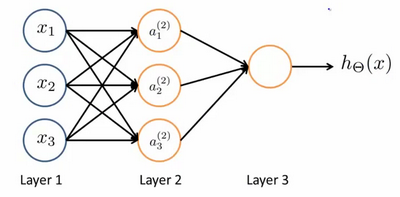
\includegraphics{image/Nerual Network.png}
    \caption{Neural Network}
\end{figure}

其中$x_1,x_2,x_3$是输入单元(input units),我们将原始数据输入给它们。$a_1,a_2,a_3$ 是中间单元,它们负责将数据进行处理,然后呈递到下一层。 最后是输出单元,它负责计算$h_\theta(x)$。

神经网络模型是许多逻辑单元按照不同层级组织起来的网络,每一层的输出变量都是下一层的输入变量。下图为一个3层的神经网络,第一层称为输入层(Input Layer),最后一层称为输出层(Output Layer),中间一层称为隐藏层(Hidden Layers)。我们为每一层都增加一个偏差单位(bias unit),相当于回归模型中的$\theta_0$

下面引入一些标记法:
\begin{itemize}
    \item $a_i^{(j)}$代表第$j$层的第$i$个激活单元,同时也可以代表这个单元的输出。
    \item $z_i^{(j)}$代表第$j$层第$i$个单元的输入。
    \item $s_j$代表第$j$层的单元个数(不包括偏置单元)。
    \item $\Theta^{(j)}$代表从第$j$层映射到第$j+1$层的权重矩阵,大小为$s_{j+1}\times (s_j+1)$
\end{itemize}

对于上图的模型:
$$
a_1 ^{(2)}=g(\sum_{i=0}^{3}\Theta_{1i}^{(1)}x_i) 
$$
$$
a_2 ^{(2)}=g(\sum_{i=0}^{3}\Theta_{2i}^{(1)}x_i)
$$
$$
a_3 ^{(2)}=g(\sum_{i=0}^{3}\Theta_{3i}^{(1)}x_i)
$$
$$
h_\Theta(x)=g(\sum_{i=1}^{3}\Theta_{1i}^{(2)}a_i)
$$

上面进行的讨论中只是将特征矩阵中的一行(一个训练实例)喂给了神经网络,我们需要将整个训练集都喂给我们的神经网络算法来学习模型。我们把这样从左到右的算法称为\textbf{前向传播算法}(forward propagation)

矩阵表示:我们令
$$
\Theta^{(1)}=\begin{bmatrix}
    \theta_{10}^{(1)} &\theta_{11}^{(1)} & \theta_{12}^{(1)} & \theta_{13}^{(1)} \\
    \theta_{20}^{(1)} &\theta_{21}^{(1)} & \theta_{22}^{(1)} & \theta_{23}^{(1)} \\   
    \theta_{30}^{(1)} &\theta_{31}^{(1)} & \theta_{32}^{(1)} & \theta_{33}^{(1)} \\ 
\end{bmatrix}
$$
那么:
$$
\begin{bmatrix}
    a_1^{(2)} \\
    a_2 ^{(2)} \\
    a_3 ^{(2)}
\end{bmatrix}=g(\Theta ^{(1)} X)
$$
插入偏置单元$a_0^{(2)}=1$:
$$
g\left(\begin{bmatrix}
    \theta_{10}^{(2)}&\theta_{11}^{(2)} &\theta_{12}^{(2)} &\theta_{13}^{(2)}
\end{bmatrix}\times \begin{bmatrix}
    a_0 ^{(2)} \\
    a_1^{(2)} \\
    a_2 ^{(2)} \\
    a_3 ^{(2)}    
\end{bmatrix}\right)=h_\theta(x)
$$
即:
$$
z ^{(j)}=\Theta ^{(j-1)}X^{(j-1)} 
$$
$$
X ^{(j)}=g(z^{(j)}) 
$$
$$
\text{Add}\quad  x_0^{(j)}=1
$$
\begin{note}
我们可以把$a_0,a_1,a_2,a_3$看成更为高级的特征值,也就是$x_0,x_1,x_2,x_3$的进化体,并且它们是由$x$与$\theta$决定的,因为是梯度下降的,所以$a$是变化的,并且变得越来越厉害,所以这些更高级的特征值远比仅仅将$x$次方厉害,也能更好的预测新数据。 这就是神经网络相比于逻辑回归和线性回归的优势。
\end{note}
\subsection{特征和直观理解}
从本质上讲,神经网络能够通过学习得出其自身的一系列特征。在普通的逻辑回归中,我们被限制为使用数据中的原始特征$x_1,\cdots,x_n$,我们虽然可以使用一些二项式项来组合这些特征,但是我们仍然受到这些原始特征的限制。在神经网络中,原始特征只是输入层,在我们上面三层的神经网络例子中,第三层也就是输出层做出的预测利用的是第二层的特征,而非输入层中的原始特征,我们可以认为第二层中的特征是神经网络通过学习后自己得出的一系列用于预测输出变量的新特征。
\newpage
\begin{example}[逻辑与(AND)]
如下图,其中$\theta_0 ^{(1)}=-30,\theta_1^{(1)}=20,\theta_2^{(1)}=20$,
$$
h_\theta(x)=g(-30+20x_1+20x_2)
$$
则验证可知:$h_\Theta(x)\approx x_1\,\text{AND}\, x_2$
\end{example}
\begin{figure}[H]
    \centering
    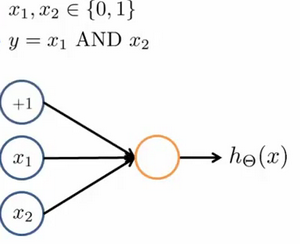
\includegraphics[width=.6\textwidth]{image/AND.png}
    \caption{逻辑与(AND)}
\end{figure}
\begin{example}[逻辑或(OR)]
$\theta_0 ^{(1)}=-10,\theta_1^{(1)}=20,\theta_2^{(1)}=20$,
$$
h_\theta(x)=g(-10+20x_1+20x_2)
$$
\end{example}
\begin{example}[逻辑非(NOT)]
$\theta_0 ^{(1)}=10,\theta_1^{(1)}=-20$,
$$
h_\theta(x)=g(10-20x_1)
$$
\end{example}

如果我们要实现异或(XNOR),即$(x_1\,\text{AND}\, x_2)\, \text{OR} \, ((\text{NOT} \,x_1)\text{AND} \\ \,(\text{{NOT}} \, x_2))$,只需要先构造一个表示$(\text{NOT} \,x_1)\text{AND}\,(\text{{NOT}} \, x_2)$的神经元(输出为$a_2^{(2)}$),然后将其和表示AND(输出为$a_1^{(2)}$)和OR的神经元(输入为$a_2^{(1)}$和$a_2^{(2)}$和偏置单元)进行组合即可。
\subsection{多类分类}
当我们有不止两种分类时,输出层可以用不同的输出神经元表示不同的类,最后选取最大的输出结果(概率最大)所属类。
\section{神经网络:学习}
\subsection{代价函数}
假设神经网络的训练样本有$m$个,每个包含一组输入$x$和一组输出信号$y$,$L$表示神经网络层数,$s_j$表示每层的neuron个数($s_L$表示输出层神经元个数)。

二元分类:$s_L=1,y\in \{0,1\}$表示输出结果属于哪一类;$K$元分类:$s_L=K,y_i=1$表示分到第$i$类$(k>2)$,此时输出$h_\theta(x)$是一个$K$维的向量。

代价函数:
$$
    J(\Theta)\!=\!-\frac{1}{m}[\sum_{i=1}^{m}\sum_{k=1}^{K}(y_k ^{(i)}\log(h_\Theta(x ^{(i)}))_k\!+(1\!-y_k ^{(i)})\log(1\!-h_\Theta(x ^{(i)}))_k]\!\newline+\frac{\lambda}{2m}\sum_{l=1}^{L-1}\sum_{i=1}^{s_l}\sum_{j=1}^{s_{l+1}}(\Theta_{ji})^2
$$

\subsection{反向传播}
为了计算代价函数的偏导数,,我们需要采用一种反向传播算法,也就是首先计算最后一层的误差,然后再一层一层反向求出各层的误差,直到倒数第二层。

\begin{definition}
定义第$l$层第$j$个单元的误差为:
$$
\delta_j^l=\frac{\partial J}{\partial z_j^l}
$$
\end{definition}

为了方便我们列出以下算式:
$$
z_j^l=\sum_{k}w_{jk}^la_k^{l-1}+b_j^l
$$
$$
a_j^l=\sigma(\sum_{k}w_{jk}^la_k^{l-1}+b_j^l)
$$
忽略正则化:
$$
J=\frac{1}{2m}\sum_x||y(x)-a^L(x)||^2
$$
\begin{lemma}
$$
\delta^L=\nabla_a J \circ \sigma'(z^L)
$$
\end{lemma}
\begin{proof}
$$
\because \delta_j^L=\frac{\partial C}{\partial z_j^L}=\frac{\partial C}{\partial a_j^L}\cdot \frac{\partial a_j^L}{\partial z_j^L} 
$$
$$
\therefore \delta^L=\frac{\partial C}{\partial a^L}\circ \frac{\partial a^L}{\partial z^L}=\nabla_a C \circ \sigma'(z^L)
$$
\end{proof}
\begin{lemma}
$$
\delta^l=((w^{l+1})^T\delta^{l+1})\circ \sigma'(z^l)
$$
\end{lemma}
\begin{proof}
$$
\begin{aligned}\because \delta_j^l=\frac{\partial C}{\partial z_j^l}
    &=\sum_k \frac{\partial C}{\partial z_k^{l+1}}\cdot\frac{\partial z_k^{l+1}}{\partial a_j^l}\cdot \frac{\partial a_j^l}{\partial z_j^l} \\
    &=\sum_k \delta_k^{l+1}\cdot\frac{\partial (\sum\limits_{k}w_{kj}^{l+1}a_j^{l}+b_k^{l+1})}{\partial a_j^l}\cdot \sigma'(z_j^l) \\
    &=\sum_k \delta_k^{l+1}\cdot w_{kj}^{l+1}\cdot \sigma'(z_j^l)
\end{aligned} 
$$
$$
\therefore \delta^l=((w^{l+1})^T\delta^{l+1})\circ \sigma'(z_j^l)
$$
\end{proof}
\begin{lemma}
$$
\frac{\partial C}{\partial w_{jk}^l}=a_k^{l-1}\delta_j^l
$$
\end{lemma}
\begin{proof}
$$
\frac{\partial C}{\partial w_{jk}^l}=\frac{\partial C}{\partial z_j^l}\cdot \frac{\partial z_j^l}{\partial w_{jk}^l}=\delta_j^l \cdot \frac{\partial (w_{jk}^l a_k^{l-1}+b_j^l)}{\partial w_{jk}^l}=a_k^{l-1}\delta_j^l
$$
\end{proof}
\begin{lemma}
$$
\frac{\partial C}{\partial b_j^l}=\delta_j^l
$$
\end{lemma}
\begin{proof}
$$
\frac{\partial C}{\partial b_j^l}=\frac{\partial C}{\partial z_j^l}\cdot \frac{\partial z_j^l}{\partial b_j^l}=\delta_j^l \cdot \frac{\partial (w_{jk}^l a_k^{l-1}+b_j^l)}{\partial b_j^l}=\delta_j^l
$$
\end{proof}

我们可以用$\Delta_{ij}^l$来表示第$l$层的第$i$个激活单元受到第$j$个参数影响而导致的误差,反向传播过程如下:
\begin{enumerate}
    \item 传入参数.
    \item 利用前向传播计算各层的输出.
    \item 初始化:$\delta^L=a^L-y$.
    \item 反向传播计算:$\Delta_{ij}^l:=\Delta_{ij}^l+a_j^l\delta_i^{l+1}$.
\end{enumerate}

求出$\Delta_{ij}^l$后就可以计算代价函数的偏导数了:
$$
D_{ij}^l=\begin{cases}
    \frac{1}{m}\Delta_{ij}^l+\frac{\lambda}{m}\Theta_{ij}^l &,j\neq 0 \\
    \frac{1}{m}\Delta_{ij}^l &,j=0
\end{cases}
$$
\subsection{梯度检验}
当我们对一个较为复杂的模型(例如神经网络)使用梯度下降算法时,可能会存在一些不容易察觉的错误,意味着,虽然代价看上去在不断减小,但最终的结果可能并不是最优解。

为了避免这样的问题,我们采取一种叫做梯度的数值检验(Numerical Gradient Checking)方法。这种方法的思想是通过估计梯度值来检验我们计算的导数值是否真的是我们要求的。对于$\theta$,以分量$\theta_1$为例,我们检验下式是否成立:
$$
\frac{\partial J}{\partial \theta_1}\approx \frac{J(\theta_1+\varepsilon,\theta_2,\cdots,\theta_n)-J(\theta_1-\varepsilon,\theta_2,\cdots,\theta_n)}{2\varepsilon}
$$
\subsection{随机初始化}
任何优化算法都需要一些初始的参数。到目前为止我们都是初始所有参数为0,这样的初始方法对于逻辑回归来说是可行的,但是对于神经网络来说是不可行的。如果我们令所有的初始参数都为0,这将意味着我们第二层的所有激活单元都会有相同的值。同理,如果我们初始所有的参数都为一个非0的数,结果也是一样的。

我们通常初始参数为$\pm \varepsilon$之间的随机值。
\section{应用机器学习的建议}
\subsection{优化策略}
\begin{itemize}
    \item 获得更多的训练样本(代价较高)。
    \item 尝试减少特征的数量。
    \item 尝试获得更多的特征
    \item 尝试增加多项式特征
    \item 尝试减少正则化程度
    \item 尝试增加正则化程度
\end{itemize}

我们不应该随机选择上面的某种方法来改进我们的算法,而是运用一些机器学习诊断法来帮助我们知道上面哪些方法对我们的算法是有效的。

\subsection{评估假设}
当我们确定学习算法的参数的时候,我们考虑的是选择参量来使训练误差最小化,有人认为得到一个非常小的训练误差一定是一件好事,但我们已经知道,仅仅是因为这个假设具有很小的训练误差,并不能说明它就一定是一个好的假设函数。而且我们也学习了过拟合假设函数的例子,所以这推广到新的训练集上是不适用的。对于简单的例子,可以对假设函数进行画图,然后观察图形趋势。但是这种方法不能推广到特征变量不止一个的情况。

为了检验算法是否过拟合,我们可以将数据分成训练集和测试集,通常用70\%的数据作为训练集,用剩下30\%的数据作为测试集。很重要的一点是训练集和测试集均要含有各种类型的数据,通常我们要对数据进行“洗牌”,然后再分成训练集和测试集。

测试集评估在通过训练集让我们的模型学习得出其参数后,对测试集运用该模型,我们有两种方式计算误差:
\begin{enumerate}
    \item 对于线性回归模型,我们利用测试集数据计算代价函数$J$.
    \item 对于逻辑回归模型,我们除了可以利用测试数据集来计算代价函数外,还可以计算误分类的比率:
\end{enumerate}
$$
err(h_\theta(x),y)=\begin{cases}
    1 \, if \, h_\theta(x) \geqslant 0.5 \, and \,y=0,\, or \, if \, h(x) \leqslant 0.5 \, and \, y=1 \\
    0 \, otherwise 
\end{cases}
$$
\subsection{模型选择和交叉验证集}
假设我们要在10个不同次数的二项式模型之间进行选择,显然越高次数的多项式模型越能够适应我们的训练数据集,但是适应训练数据集并不代表着能推广至一般情况,我们应该选择一个更能适应一般情况的模型。我们需要使用交叉验证集来帮助选择模型。 即:使用60\%的数据作为训练集,使用20\%的数据作为交叉验证(Cross Validation )集,使用20\%的数据作为测试集。模型选择的方法为:
\begin{enumerate}
    \item 使用训练集训练出10个模型。
    \item 用10个模型分别对交叉验证集计算得出交叉验证误差(代价函数的值)。
    \item 选取代价函数值最小的模型。
    \item 用步骤3中选出的模型对测试集计算得出推广误差(代价函数的值)。
\end{enumerate}
\begin{note}
训练误差:
$$
J_{train}(\theta)=\frac{1}{2m}\sum_{i=1}^m(h_\theta(x^{(i)})-y^{(i)})^2
$$
交叉验证误差:
$$
J_{cv}(\theta)=\frac{1}{2m_{cv}}\sum_{i=1}^{m_{cv}}(h_\theta(x_{cv}^{(i)})-y_{cv}^{(i)})^2
$$
推广误差:
$$
J_{test}(\theta)=\frac{1}{2m_{test}}\sum_{i=1}^{m_{test}}(h_\theta(x_{test}^{(i)})-y_{test}^{(i)})^2
$$
\end{note}
\subsection{诊断偏差和方差}
当你运行一个学习算法时,如果这个算法的表现不理想,那么多半是出现两种情况:要么是偏差比较大,要么是方差比较大。换句话说,出现的情况要么是欠拟合,要么是过拟合问题,高偏差和高方差的问题基本上来说是欠拟合和过拟合的问题。

我们通常会通过将训练集和交叉验证集的代价函数误差与多项式的次数绘制在同一张图表上来帮助分析:
\begin{figure}[H]
    \centering
    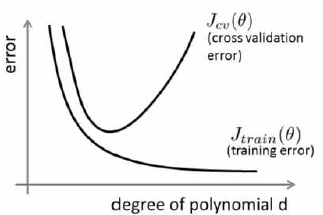
\includegraphics{image/error.png}
    \caption{Error vs. degree}
\end{figure}

对于训练集,当$d$较小时,模型拟合程度更低,误差较大;随着$d$的增长,拟合程度提高,误差减小。 对于交叉验证集,当$d$较小时,模型拟合程度低,误差较大;但是随着$d$的增长,误差呈现先减小后增大的趋势,转折点是我们的模型开始过拟合训练数据集的时候。 所以:训练集误差和交叉验证集误差近似时:偏差/欠拟合;交叉验证集误差远大于训练集误差时:方差/过拟合。

\subsection{正则化和偏差/方差}
在我们在训练模型的过程中,一般会使用一些正则化方法来防止过拟合。但是我们可能会正则化的程度太高或太小了,即我们在选择λ的值时也需要思考与刚才选择多项式模型次数类似的问题。

我们选择一系列的想要测试的$\lambda$值,通常是 0-10之间的呈现2倍关系的值,然后采取7.3中的方法。如果仿照之前的方式画出误差和$\lambda$之间的函数图像,会发现当$\lambda$较小时,训练集误差较小(过拟合)而交叉验证集误差较大;随着$\lambda$的增加,训练集误差不断增加(欠拟合),而交叉验证集误差则是先减小后增加。
\subsection{学习曲线}
学习曲线就是一种很好的工具,我经常使用学习曲线来判断某一个学习算法是否处于偏差、方差问题。学习曲线是学习算法的一个很好的合理检验(sanity check)。学习曲线是将训练集误差和交叉验证集误差作为训练集样本数量($m$)的函数绘制的图表。 即,如果我们有100行数据,我们从1行数据开始,逐渐学习更多行的数据。思想是:当训练较少行数据的时候,训练的模型将能够非常完美地适应较少的训练数据,但是训练出来的模型却不能很好地适应交叉验证集数据或测试集数据。

在欠拟合情况下,可以发现无论训练集多么大误差都不会有太大改观;而在过拟合情况下,训练集误差将会比较平缓且很小,而增加更多数据能显著减小交叉验证误差。
\subsection{类偏斜的误差度量}
使用一个合适的误差度量值,这有时会对于你的学习算法造成非常微妙的影响,这件重要的事情就是偏斜类(skewed classes)的问题。类偏斜情况表现为我们的训练集中有非常多的同一种类的样本,只有很少或没有其他类的样本。

例如我们希望用算法来预测癌症是否是恶性的,在我们的训练集中,只有0.5\%的实例是恶性肿瘤。假设我们编写一个非学习而来的算法,在所有情况下都预测肿瘤是良性的,那么误差只有0.5\%。然而我们通过训练而得到的神经网络算法却有1\%的误差。这时,误差的大小是不能视为评判算法效果的依据的。 

我们可以将算法预测的结果分成四种情况:
\begin{enumerate}
    \item 正确肯定(True Positive,TP):预测为真,实际为真.
    \item 正确否定(True Negative,TN):预测为假,实际为假.
    \item 错误肯定(False Positive,FP):预测为真,实际为假.
    \item 错误否定(False Negative,FN):预测为假,实际为真
\end{enumerate}

\begin{definition}[查全率和查准率]
查全率(Recall,R)=$\frac{\text{TP}}{\text{TP+FN}}$,本例中为在所有实际上有恶性肿瘤的病人中,成功预测有恶性肿瘤的病人的百分比;查准率(Precision,P)=$\frac{\text{TP}}{\text{TP+TN}}$,本例中为在所有我们预测有恶性肿瘤的病人中,实际上有恶性肿瘤的病人的百分比。
\end{definition}

如何权衡查准率和查全率:在logistic回归中我们通常使用0.5作为预测的阈值。但如果希望更高的查准率,我们可以使用比0.5更大的阀值,如0.7,0.9。这样做我们会减少错误预测病人为恶性肿瘤的情况,同时却会增加未能成功预测肿瘤为恶性的情况。 如果我们希望提高查全率,尽可能地让所有有可能是恶性肿瘤的病人都得到进一步地检查、诊断,我们可以使用比0.5更小的阀值,如0.3。
\begin{note}
一种选择阈值的方式是让F1 Score最大,计算公式为:
$$
\text{F1Score}=\frac{2PR}{P+R}
$$
\end{note}
\section{支持向量机}
\subsection{代价函数}
在逻辑回归中,如果$y=1$,我们期望$h(x) \approx 1,\theta^T x>>0$;如果$y=0$,我们期望$h(x) \approx 0,\theta^T x<<0$。

我们可以采用hinge loss来代替logistic回归中的损失函数:
$$
\ell_{hinge}(z)=\max(1-z,0)\approx \log(\frac{1}{1+e^{z}})
$$
代价函数:
$$
J(\theta)=-\sum_{i=1}^{m}[y^i\ell_1(\theta^Tx^i)+(1-y^i)\ell_0(\theta^Tx^i)]+\frac{\lambda}{2}\sum_{i=0}^{n}\theta_i^2
$$
在SVM中我们习惯把代价函数写成下面这种形式:
$$
J(\theta)=C\sum_{i=1}^{m}[y^i\ell_1(\theta^Tx^i)+(1-y^i)\ell_0(\theta^Tx^i)]+\frac{1}{2}\sum_{i=0}^{n}\theta_i^2
$$

最后有别于逻辑回归输出的概率,支持向量机直接输出1或0。因此,当$\theta^Tx$大于或者等于0时,这个假设函数会预测1,反之会输出0。这就是支持向量机数学上的定义。
$$
h_\theta(x)=\begin{cases}
    1 & \text{if} \, \theta ^T x \geqslant 0 \\
    0 &\text{otherwise}
\end{cases}
$$
\subsection{大间距分类器}
观察代价函数的形式可以发现,当我们有一个正样本$y=1$时,只有$\theta^T x \leqslant 1$时$cost_0(z)$才为0。因此相比于逻辑回归,支持向量机的要求更高,不仅仅要能正确分开输入的样本,即不仅仅要求$\theta^Tx>0$,我们需要的是它比0值大很多,比如大于等于1;在样本为负向类时也希望它比0小很多,比如我希望它小于等于-1,这就相当于在支持向量机中嵌入了一个额外的安全因子,或者说安全的间距因子。

如果我们让$C$非常大,那么当优化代价函数时我们将试图让下式保持成立:
$$
\theta^T x_i \geqslant 1,y=1
$$
$$
\theta^T x_i \leqslant -1,y=0
$$
在直观上就是让不同类之间尽可能保持最大间距。
\subsection{数学推导}
样本点到边界的距离:
$$
\gamma_i=y_i (\frac{\omega^T}{||\omega||}\cdot x_i+\frac{b}{||\omega||})
$$
定义:
$$
\gamma=\min_{i=1,2,\cdots,N}\gamma_i
$$
SVM的目的就是$\max\limits_{\omega,b} \gamma$,且:
$$
y_i (\frac{\omega}{||\omega||}\cdot x_i+\frac{b}{||\omega||})\geqslant \gamma
$$
即:
$$
y_i (\frac{\omega}{||\omega||\gamma}\cdot x_i+\frac{b}{||\omega||\gamma})\geqslant 1
$$
重新定义:
$$
\omega=\frac{\omega}{||\omega||\gamma}
$$
$$
b=\frac{b}{||\omega||\gamma}
$$
因此欲最大化$\gamma$,只需要最小化$\frac{1}{2}||w||^2$。优化目标变为:
$$
\min_{\omega,b}\frac{1}{2}||\omega||^2,s.t.y_i(\omega\cdot x_i+b)\geqslant 1
$$
\begin{definition}[凸集]
$\mathbf{C}$为凸集(convex set)当且仅当:
$$
\forall x,y \in \mathbf{C},\forall \Theta \in [0,1],\Theta x+(1-\Theta)y \in \mathbf{C}
$$
\end{definition}
\begin{definition}[凸优化问题]
$f(x)$是凸函数,
$$
\min f(x),s.t. x\in \mathbf{C}
$$
\end{definition}
那么SVM的优化问题属于(二次)凸优化问题。更一般的,我们研究如下问题:
$$
\min_x f(x),s.t.h_i(x)=0,g_i(x)\leqslant 0
$$      
\begin{theorem}[KKT条件]
对于上述约束优化问题,定义Lagrangian函数:
$$
L(x,\lambda,\mu)=f(x)+\sum_{i=1}^m \lambda_i h_i(x)+\sum_{j=1}^p \mu_j g_j(x)
$$
那么非线性规划问题最优点的必要条件(Karush-Kuhn-Tucker Conditions)是:
$$
\begin{cases}
\nabla_x L=0 \\
h_i(x)=0,i=1,\cdots,m \\
g_i(x)\leqslant 0,i=1,\cdots,p \\
\mu_i \geqslant 0,i=1,\cdots,p \\
\mu_i g_i(x)=0,i=1,\cdots,p
\end{cases}
$$
\end{theorem}
我们定义上述问题为原始问题,如果$x$违反了某些约束,我们令$L(x,\lambda,\mu)=+\infty$,则:
$$
\min_x \max_{\lambda,\mu} L(x,\lambda,\mu)=\min_{x^*} f(x^*)
$$
其中$x^*$满足约束。定义对偶问题:
$$
\max_{\lambda,\mu} \min_x L(x,\lambda,\mu),s.t. \alpha_i \geqslant 0
$$
对偶问题是原始问题的下界,即:
$$
\max_{\lambda,\mu} \min_x L(x,\lambda,\mu) \leqslant \min_x \max_{\lambda,\mu} L(x,\lambda,\mu)
$$
该不等式被称为弱对偶性(weak duality),强对偶性需要等号成立:
\begin{theorem}[slater条件]
原始问题为凸优化问题,即$f(x),g(x)$为凸函数,$h(x)$为仿射函数(线性),且可行域中至少有一点使不等式约束严格成立时,强对偶性成立,对偶问题等价于原始问题。
\end{theorem}

对于SVM问题:Lagrangian函数为:
$$
L(\omega,b,\alpha)=\frac{1}{2}||\omega||^2+\sum_{i=1}^{m}\alpha_i(1-y_i(\omega^Tx_i+b)),\alpha_i \geqslant 0
$$
原始问题$\min\limits_{\omega,b}\max\limits_{\alpha} L(\omega,b,\alpha)$的外层出现了两个变量,运算量过大,同时容易发现,该问题满足强对偶条件,因此不妨考虑其对偶问题:
$$
\max_\alpha \min_{\omega,b} L(\omega,b,\alpha)
$$
$$
\frac{\partial L}{\partial \omega}=\omega-\sum_{i=1}^{m}\alpha_i y_i x_i=0
$$
$$
\frac{\partial L}{\partial b}=-\sum_{i=1}^{m}\alpha_i y_i=0
$$
代入可得其对偶问题:
$$
\max_\alpha \sum_{i=1}^{m}\alpha_i-\frac{1}{2}\sum_{i=1}^{m}\sum_{j=1}^{m}\alpha_i\alpha_jy_iy_jx_i^Tx_j,s.t. \sum_{i=1}^{m}\alpha_iy_i=0
$$
此时
$$
f(x)=\omega^Tx+b=\sum_{i=1}^m \alpha_i y_i x_i x+b
$$
且上述过程还需满足KKT条件,即 :
$$
\begin{cases}
    \alpha_i \geqslant 0 \\
    y_if(x_i)-1 \geqslant 0 \\
    \alpha_i(y_if(x_i)-1)=0
\end{cases}
$$
SVM的数学推导未完待续。
\subsection{核函数}
我们可以使用高级数的多项式模型来解决无法用直线进行分隔的分类问题,可能采用如下形式:
$$
h_\theta(x)=\theta_0+\theta_1x_1+\theta_2x_2+\theta_3 x_1^2+\cdots
$$
可以用新的一系列特征来替换模型中的每一项:
$$
f_1=x_2,f_2=x_2,f_3=x_1^2,\cdots
$$
有没有更好的方法来构造这些特征(因为可能存在特征过多等问题)?我们可以利用核函数来计算出新的特征。

给定一个训练样本$x$,我们利用$x$的各个特征与我们预先选定的地标(landmarks)$\{l_i\}$的近似程度来选取新的特征$\{f_i\}$。例如:
$$
f_1=sim(x,l_1)=e^{-\frac{||x-l_1||^2}{2\sigma^2}}
$$

我们通常是根据训练集的数量选择地标的数量,即如果训练集中有$m$个样本,则我们选取$m$个地标,并且令:$l_1=x_1,\cdots,l_m=x_m$。这样做的好处在于:现在我们得到的新特征是建立在原有特征与训练集中所有其他特征之间距离的基础之上的,即:
$$
f^{(i)}=\begin{bmatrix}
    f_0^{(i)}=1 \\
    f_1^{(i)}=sim(x^{(i)},l_1) \\
    \vdots \\
    f_i^{(i)}=1 \\
    \vdots \\
    f_m^{(i)}=sim(x^{(i)},l_m)
\end{bmatrix}
$$

这种换算方式被称作高斯核函数,其本质是把一个空间映射到无穷维。除此之外还有多项式核函数,字符串核函数吗,卡方核函数,直方图交集核函数等。

\section{聚类}
聚类是典型的无监督学习,旨在根据数据的分布特征将其分类。
\subsection{K-Means 算法}
K-均值是最普及的聚类算法,算法接受一个未标记的数据集,然后将数据聚类成不同的组,假设我们想要将数据聚类成n个组,其方法为:
\begin{enumerate}
    \item 首先选择$K$个随机的点,称为聚类中心(cluster centroids)。
    \item 对于数据集中的每一个数据,按照距离$K$个中心点的距离,将其与距离最近的中心点关联起来,与同一个中心点关联的所有点聚成一类。
    \item 计算每一个组的平均值,将该组所关联的中心点移动到平均值的位置。
    \item 重复上述各步直至收敛.
\end{enumerate}
\subsection{优化目标}
K-均值最小化问题,是要最小化所有的数据点与其所关联的聚类中心点之间的距离之和,因此 K-均值的代价函数(又称畸变函数 Distortion function)为:
$$
J(c^1,\cdots,c^m,\mu_1,\cdots,\mu_K)=\frac{1}{m}\sum_{i=1}^{m}(||x^i-\mu_{c^i}||)^2
$$
其中$c^i$表示与第$i$个实例数据最近的聚类中心的索引,$\mu_i$表示聚类中心,很明显K-均值算法能够减小代价函数。
\subsection{随机初始化}
\begin{enumerate}
    \item 选择$K<m$,即聚类中心点的个数要小于所有训练集实例的数量。
    \item 随机选择$K$个训练实例,然后令$K$个聚类中心分别与这$K$个训练实例相等
\end{enumerate}

K-均值的一个问题在于,它有可能会停留在一个局部最小值处,而这取决于初始化的情况。为了解决这个问题,我们通常需要多次运行K-均值算法,每一次都重新进行随机初始化,最后再比较多次运行K-均值的结果,选择代价函数最小的结果。这种方法在$K$较小的时候(2-10)还是可行的,但是如果$K$较大,这么做也可能不会有明显地改善。
\subsection{选择聚类数}
通常是需要根据不同的问题,人工进行选择的。选择的时候思考我们运用K-均值算法聚类的动机是什么,然后选择能最好服务于该目的标聚类数。一个方法叫做肘部法则:作出代价函数和聚类数的函数关系图,然后选择图像的转折点。

簇内不相似度:计算样本$i$到同簇其它样本的平均距离$a_i$,应尽可能小;簇间不相似度:计算样本$i$到其它簇$C_j$的所有样本的平均距离$b_{ij}$,$b_i$定义为:
$$
b_i=\min (b_{i1},b_{i2},\cdots,b_{iK})
$$
应尽可能大。轮廓系数$s_i$定义为:
$$
s_i=\frac{b_i-a_i}{\max(a_i,b_i)}
$$
其值越接近1说明$i$聚类越合理,近似为0说明在边界,近似为-1说明应该被分到其他的簇。
\section{降维}
\subsection{数据压缩和可视化}
假如数据集的样本有两个特征,都表示物体长度,因此特征是高度冗余的。因此我们不妨只用一个维度来描述样本。再比如三维数据降维:
\begin{figure}[H]
    \centering
    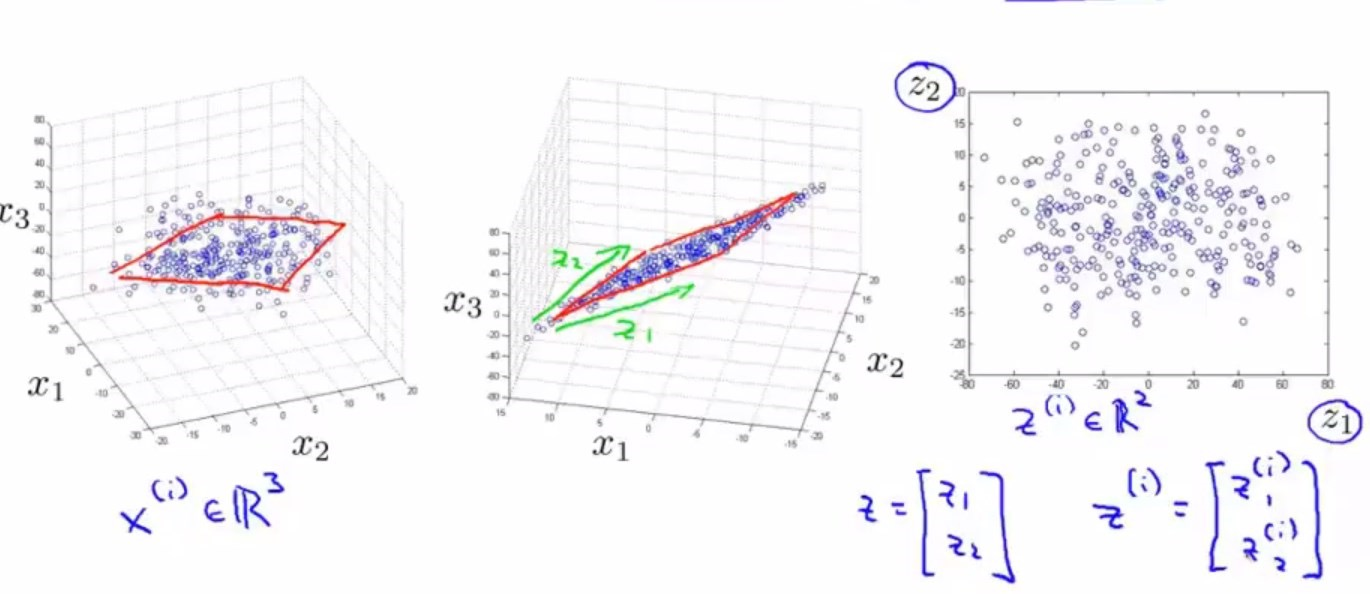
\includegraphics[width=12cm,height=7cm]{image/reduce dimension.jpeg}
    \caption{降维}
\end{figure}

降维除了能数据压缩,还可以进行数据的可视化。
\subsection{主成分分析}
对于降维问题,最流行的算法是PCA(Principal Component Analysis)。PCA的目的是找到一个低维空间,将数据投影在上面,使得数据与投影点之间的垂直距离(欧氏距离)的平方和最小。即找出$k$个向量$(u_1,\cdots,u_k)$,将数据投影到这$k$个向量展开的线性子空间上,使得误差函数最小。另外在PCA之前通常要均值归一化和特征规范化。

\subsubsection{数学原理}
\begin{definition}[协方差]
对于随机变量$X,Y$,二者的协方差定义如下:
$$
Cov[X,Y]=E[(X-\mu)(Y-v)]
$$
其中$\mu$是$X$的期望,$v$是$Y$的期望。
\end{definition}
引入协方差矩阵,第$i$行$j$列表示$X_i$和$X_j$的协方差,对角线上表示自身的方差,协方差矩阵是对称矩阵。

降维策略:一是考虑除掉特征之间的相关性,二是在彼此无关的特征集中舍弃掉不必要的特征,实现数据的特征维数降维。首先如何构造无关的特征?将协方差矩阵变换成对角矩阵。
$$
Cov[X,Y]=\frac{1}{n-1}\sum_{i=1}^n (x_i-\mu)(y_i-v)
$$
通过零均值化处理:
$$
Cov[X,Y]=\frac{1}{n-1}x_iy_i
$$

以两个特征为例,写出零均值化处理的协方差矩阵:
$$
C=\frac{1}{n-1}\begin{bmatrix}
    \sum\limits_{i=1}^n x_i^2 & \sum\limits_{i=1}^n x_iy_i  \\
    \sum\limits_{i=1}^n y_ix_i & \sum\limits_{i=1}^n y_i^2
\end{bmatrix}
$$
令
$$
A=\begin{bmatrix}
    x_1 &x_2 &\cdots &x_n \\
    y_1 &y_2 &\cdots &y_n
\end{bmatrix}
$$
那么可以发现:
$$
C=AA^T
$$
因此协方差矩阵是对称且正定的满秩矩阵。令$C$的$n$个标准正交特征向量组成的矩阵为$P$,那么$PCP^T$即为要求的对角矩阵。令新的特征构成的矩阵为$PA$,则得到了无关的特征,在此基础上进行降维。

具体保留哪些维度我们的判定标准是方差,方差越大,表明数据的离散程度大,所含信息量大,我们保留这个特征。比如说把二维特征映射到一维,我们定义主成分贡献率:
$$
\frac{\lambda_1}{\lambda_1+\lambda_2}
$$
如果主成分贡献率高于50\%,说明效果还不错。
\begin{note}
对于$n$维映射到$k$维,样本数据矩阵A为$m\times n$,可以直接对$A$作奇异值分解$A=U\Sigma V$,得到的$\Sigma$矩阵中前$k$列奇异值(最大的$k$列)对应$U$的前$k$列列向量即为所求。
\end{note}
\subsection{选择主成分的数量}
定义降维矩阵$U_{\rm{reduce}}=[u^1,\cdots,u^k]$,$k$维的新特征$z^i=U_{\rm{reduce}}^T x_i$,定义投影误差:
$$
\frac{1}{m}\sum_{i=1}^m ||x^i-x_{\rm{approx}}^i||^2
$$
其中$x_{\rm{approx}}^i=U_{\rm{reduce}}z^i$,数据的总方差:
$$
\frac{1}{m}\sum_{i=1}^m ||x^i||^2
$$
在选择$k$时一个常见的经验主导的方法是选择使:
$$
\frac{\frac{1}{m}\sum\limits_{i=1}^m ||x^i-x_{\rm{approx}}^i||^2}{\frac{1}{m}\sum\limits_{i=1}^m ||x^i||^2} \leqslant 0.01
$$
的最小的$k$值,专业的表达是"99\%的方差得到了保留"。
\section{异常检测}
\begin{example}
飞机引擎生产的时候需要进行质量检测,假如已经生产了$m$个引擎,并得到了一个数据集$x_1,\cdots,x_m$,假定数据集是正常的,我们希望知道新的数据$x_{\rm{test}}$是否具有某种异常。我们构建的模型应该根据测试数据的位置告诉我们其属于一组数据的可能性$p(x)$。
\end{example}

这种方法称作密度估计:
$$
\text{if} \quad p(x)
\begin{cases}
    < \varepsilon &\rm{abnormal} \\
    \geqslant \varepsilon &\rm{normal}
\end{cases}
$$
异常检测主要用来识别欺骗。例如在线采集而来的有关用户的数据,一个特征向量中可能会包含如:用户多久登录一次,访问过的页面,在论坛发布的帖子数量,甚至是打字速度等。尝试根据这些特征构建一个模型,可以用这个模型来识别那些不符合该模式的用户。

再一个例子是检测一个数据中心,特征可能包含:内存使用情况,被访问的磁盘数量,CPU的负载,网络的通信量等。根据这些特征可以构建一个模型,用来判断某些计算机是不是有可能出错了。
\subsection{高斯分布}
$$
p(x,\mu,\sigma^2)=\frac{1}{\sqrt{2\pi}\sigma}\exp{(-\frac{(x-\mu)^2}{2\sigma^2})}
$$
机器学习中对于方差通常只除以$m$,而非统计学中的$m-1$
\subsection{算法}
给定一个数据集$\{x^1,\cdots,x^m\}$,对于每个特征分别计算$\mu_j=\frac{1}{m}\sum\limits_{i=1}^m x_j^i$,方差$\sigma_j^2=\frac{1}{m}\sum\limits_{i=1}^m (x_j^i-\mu_j)^2$.

完成参数估计之后引入一个新的样本,计算如下式子的值:
$$
p(x)=\prod_{j=1}^n p(x_j,\mu_j,\sigma_j^2)=\prod_{j=1}^n \frac{1}{\sqrt{2\pi}\sigma_j}\exp{(-\frac{(x_j-\mu_j)^2}{2\sigma_j^2})}
$$
如果$p(x)<\varepsilon$,说明样本异常。

异常检测过程是无监督学习,评估异常检测的过程如下:
\begin{enumerate}
    \item 用训练集数据去拟合分布模型$p(x)$.
    \item 对交叉验证集或者测试集上的任一样本预测其$y$值.
    \item 考虑到这是一个偏斜类,因为实际生产中,异常的总是少数,所以考虑到之前学过的查准率和召回率的应用,或者F1值.
    \item 根据评估度量查准率和召回率的应用,或者F1值来选择$\varepsilon$
\end{enumerate}

相比于监督学习,异常检测的异常数量稀少,或者是难以学习,即其数据集十分偏斜。
\subsection{特征选择}
在异常检测中,我们所使用的特征常常都是服从高斯分布的,如果特征不服从,异常检测算法也可以正常工作,但是如果将数据转换为高斯分布的话,从感觉上或者经验上来说,算法会运行得更好。

业内常对特征采用变换:$x_j=\log(x_j+c),c\geqslant 0$或者$x_j=x_j^c,c\in (0,1)$,函数图像会更像高斯分布。

一个常见的问题是一些异常的数据可能也会有较高的$p(x)$值,因而被算法认为是正常的。这种情况下误差分析能够帮助我们,我们可以分析那些被算法错误预测为正常的数据,思考能够能从问题中发现我们需要增加一些新的特征,增加的新特征能够提高学习算法的性能。

我们通常可以通过将一些相关的特征进行组合,来获得一些新的更好的特征(异常数据的该特征值异常地大或小),例如,在检测数据中心的计算机状况的例子中,我们可以用CPU负载与网络通信量的比例作为一个新的特征,如果该值异常地大,便有可能意味着该服务器是陷入了一些问题中。
\subsection{多元高斯分布}
假使我们有两个相关的特征,而且这两个特征的值域范围比较宽,这种情况下,一般的高斯分布模型可能不能很好地识别异常数据。其原因在于,一般的高斯分布模型尝试的是去同时抓住两个特征的偏差,因此拟合出一个比较大的判定边界。

在一般的高斯分布模型中我们累乘$p(x)$,而在多元高斯分布中我们首先计算所有特征的均值,然后计算协方差矩阵:
$$
\Sigma=\frac{1}{m}(X-\mu)^T(X-\mu)
$$
$$
p(x)=\frac{1}{(\sqrt{2\pi})^n |\Sigma|^{\frac{1}{2}}}e^{-\frac{1}{2}(x-\mu)^T\Sigma^{-1}(x-\mu)}
$$
可以证明的是,原本的高斯分布模型是多元高斯分布模型的一个子集,如果协方差矩阵只在对角线的单位上有非零的值时,即为原本的高斯分布模型了。

使用多元高斯分布模型时要保证$m>n$,通常要$m>10n$。
\section{推荐系统}
\begin{example}
假使我们是一个电影供应商,我们有5部电影和4个用户,我们要求用户为电影打分。前三部电影是爱情片,后两部则是武打片,并且没有一个用户给所有的电影都打过分。我们希望构建一个算法来预测他们每个人可能会给他们没看过的电影打多少分,并以此作为推荐的依据。
\end{example}
下面引入一些标记:
\begin{enumerate}
    \item $n_u$代表用户的数量;
    \item $n_m$代表电影的数量;
    \item $r(i,j)$:如果用户$j$给电影$i$评过分则$r(i,j)=1$;
    \item $y^{(i,j)}$代表用户$j$给电影$i$的评分;
    \item $m_j$代表用户$j$评过分的电影的总数.
\end{enumerate}
\subsection{基于内容的推荐系统}
在我们的例子中,我们可以假设每部电影都有两个特征,如$x_1$代表电影的浪漫程度,$x_2$代表电影的武打程度,则每部电影都有其特征向量。假设采用线性回归模型:
对于用户$j$和电影$i$,我们预测评分为$(\theta^{(j)})^Tx^{(i)}$,针对用户$j$,代价函数:
$$
\min_{\theta^{(j)}} \frac{1}{2}\sum_{i:r(i,j)=1}((\theta^{(j)})^Tx^{(i)}-y^{(i,j)})^2+\frac{\lambda}{2}\sum_{k=1}^n(\theta_k^{(j)})^2
$$
而对所有用户:
$$
\min_{\theta^{(1)},\cdots,\theta^{(n_u)}} \frac{1}{2}\sum_{j=1}^{n_u}\sum_{i:r(i,j)=1}((\theta^{(j)})^Tx^{(i)}-y^{(i,j)})^2+\frac{\lambda}{2}\sum_{j=1}^{n_u}\sum_{k=1}^n(\theta_k^{(j)})^2
$$
梯度下降步骤如下:
$$
\theta_k^{(j)}:=\theta_k^{(j)}-\alpha\left(\sum_{i:r(i,j)=1}((\theta^{(j)})^Tx^{(i)}-y^{(i,j)}x_k^{(i)}) +\lambda \theta_k^{(j)}\right),k\neq 0
$$
$$
\theta_k^{(j)}:=\theta_k^{(j)}-\alpha\sum_{i:r(i,j)=1}((\theta^{(j)})^Tx^{(i)}-y^{(i,j)}x_k^{(i)}),k=0
$$
\subsection{协同过滤}
在之前的基于内容的推荐系统中,对于每一部电影,我们都掌握了可用的特征,使用这些特征训练出了每一个用户的参数。相反地,如果我们拥有用户的参数,我们可以学习得出电影的特征。
$$
\min_{x^{(1)},\cdots,x^{(n_m)}}\frac{1}{2}\sum_{i=1}^{n_m}\sum_{j:r(i,j)=1}((\theta^{(j)})^Tx^{(i)}-y^{(i,j)})^2+\frac{\lambda}{2}\sum_{i=1}^{n_m}\sum_{k=1}^n(x_k^{(i)})^2
$$
我们的优化目标便改为同时针对$x$和$\theta$进行:
\begin{footnotesize}
$$
  J(x^{(1)},\cdots,x^{(n_m)},\theta^{(1)},\cdots,\theta^{(n_u)})=\frac{1}{2}\sum_{(i:j):r(i,j)=1}((\theta^{(j)})^Tx^{(i)}-y^{(i,j)})^2+\frac{\lambda}{2}\sum_{i=1}^{n_m}\sum_{k=1}^n(x_k^{(i)})^2+\frac{\lambda}{2}\sum_{k=1}^n(\theta_k^{(j)})^2  
$$
\end{footnotesize}
需要注意的是,使用结合之后的目标优化函数,将不再需要$x_0=1$这一项。
梯度下降(下式可能有误):
$$
\theta_k^{(j)}:=\theta_k^{(j)}-\alpha\left(\sum_{i:r(i,j)=1}((\theta^{(j)})^Tx^{(i)}-y^{(i,j)}x_k^{(i)}) +\lambda \theta_k^{(j)}\right)
$$
$$
x_k^{(j)}:=x_k^{(j)}-\alpha\left(\sum_{i:r(i,j)=1}((\theta^{(i)})^Tx^{(j)}-y^{(i,j)}\theta_k^{(i)}) +\lambda x_k^{(j)}\right)
$$
\subsection{低秩矩阵分解}
我们可以把用户对电影的评分存到矩阵中,然后训练出评分矩阵。

学习出特征向量之后,衡量电影的相似性只需要计算两个向量的距离:$||x^{(i)}-x^{(j)}||$,推荐时只需要找出和用户喜欢看的电影最相似的即可。
\begin{note}
均值归一化:如果我们新增一个没有对任何电影评分的用户,我们首先要对结果矩阵进行均值归一化,对于新用户,模型认为她给每部电影的评分都是平均分。因为如果没有采用平均打分,为了最小化代价函数,新用户会给每个电影打出0分。
\end{note}
\section{大规模机器学习}
学习曲线(learning curves),可以帮助我们判断是否有必要使用海量的数据集。
\subsection{随机梯度下降和小批量梯度下降}
对于普通的梯度下降算法而言,在每次更新参数值的时候都会对$m$个样本求和,所以业内也常称之为批量梯度下降。如果$m$特别大,那么这个计算代价就会十分大,因为每次更新都会对$m$个实数求和。

随机梯度下降算法(SGD,Stochastic Gradient Descent)为:首先对数据集随机“洗牌”,然后对下述步骤重复1-10次:

\noindent \textbf{for i=1:m}
$$
\theta_j:=\theta_j-\alpha (h_\theta(x^{(i)}-y^{(i)})x_j^{(i)}
$$

随机梯度下降算法在每一次计算之后便更新参数$\theta$,而不需要首先将所有的训练集求和,在梯度下降算法还没有完成一次迭代时,随机梯度下降算法便已经走出了很远。但是这样的算法存在的问题是,不是每一步都是朝着”正确”的方向迈出的。因此算法虽然会逐渐走向全局最小值的位置,但是可能无法站到那个最小值的那一点,而是在最小值点附近徘徊。

小批量梯度下降算法是介于批量梯度下降算法和随机梯度下降算法之间的算法,每计算常数$b$次训练实例,便更新一次参数$\theta$:

\noindent \textbf{for i=1:m\{}
$$
\theta_j:=\theta_j-\alpha \frac{1}{b}\sum_{k=i}^{i+b-1} (h_\theta(x^{(k)}-y^{(k)})x_j^{(k)}
$$
$$i+=10$$
\textbf{\}}

通常我们会令$b$在 2-100之间。这样做的好处在于,我们可以用向量化的方式来循环$b$个训练实例。
\subsection{随机梯度下降的收敛}
我们介绍随机梯度下降算法的调试,以及学习率$\alpha$的选取。

在随机梯度下降中,我们在每一次更新$\theta$之前都计算一次代价,然后每$x$次迭代后,求出这次对训练实例计算代价的平均值,然后绘制这些平均值与$x$次迭代的次数之间的函数图表。根据图像调整学习率,我们也可以令学习率随着迭代次数的增加而减小,例如令:
$$
\alpha=\frac{C_1}{No.+C_2}
$$
\subsection{在线学习}
假使我们正在经营一家物流公司,每当一个用户询问从地点A至地点B的快递费用时,我们给用户一个报价,该用户可能选择接受($y=1$)或不接受($y=0$)。

现在,我们希望构建一个模型,来预测用户接受报价使用我们的物流服务的可能性。因此报价 是我们的一个特征,其他特征为距离,起始地点,目标地点以及特定的用户数据。模型的输出是:$p(y=1)$。

在线学习的算法与随机梯度下降算法有些类似,我们对单一的实例进行学习,而非对一个提前定义的训练集进行循环。一旦对一个数据的学习完成了,我们便可以丢弃该数据,不需要再存储它了。这种方式的好处在于,我们的算法可以很好的适应用户的倾向性,算法可以针对用户的当前行为不断地更新模型以适应该用户。

完结撒花!
\end{document}